\section{Introduction}
In this chapter we are going to present some recent work and research that was done regarding skin cancer detection and classification using machine learning, we are going to explore the various methods, tools, new ideas and challenges that were handled by researchers in the hope of getting a clear understanding of the problem and how to go about solving it depending on each one's conditions, requirements and goals.



\section{Skin Cancer Detection and Classification Using Machine Learning}
\begin{description}
    \item [Proposed methodology] \hfill \\
    The proposed methodology in this article ~\cite{Krishna2020} uses a 6-step process (input data - preprocessing - segmentation - feature extraction - classification - output data).
    \item [Input data] \hfill \\ 
        Dermoscopic images from the ISIC ( International Skin Imaging Collaboration) 2019 challenge containing 8 classes of skin lesions, and for simplicity reasons only 800 images out of, 25000 are used.
    
    \item [Preprocessing] \hfill \\
        Because of the heterogeneity of the input data, a preprocessing step is required to enhance the quality of images and remove irrelevant parts. The main techniques used here are gray scale conversion and the application of the Gaussian and median filter for noise removal and enhancement, and for the unwanted hair they applied the Dull Razor method (a preprocessing algorithm), as shown in figure ~\ref{fig:Preprocessing}.

    \item [Segmentation] \hfill \\
        Segmentation is used to extract the region of interest and for that they used a k-means clustering algorithm as shown in figure \ref{fig:segmentation}.
        
    \item [Feature extraction] \hfill \\
        For this they used 2 well known methods, ABCD method and GLCM. ABCD is used in dermatological applications and diagnosis for skin lesions such as melanomas, and it is the abbreviation of Asymmetry, Border, Color and Diameter. Grey Level Co-occurrence Matrix (GLCM) is used for texture analysis, other features are also used in addition to these 2 methods for further classification such as Autocorrelation, correlation, Standard vector...etc.
    
    \item [Classification] \hfill \\
        For classification, they used MSVM (Multi-class Support vector machine) machine learning algorithm, they used training and testing ratios of 70:30 and obtained an accuracy of 96.25\% and the confusion matrix shown in figure \ref{fig:confusion-matrix}.
\end{description}

\begin{figure}[htbp]
\begin{center}
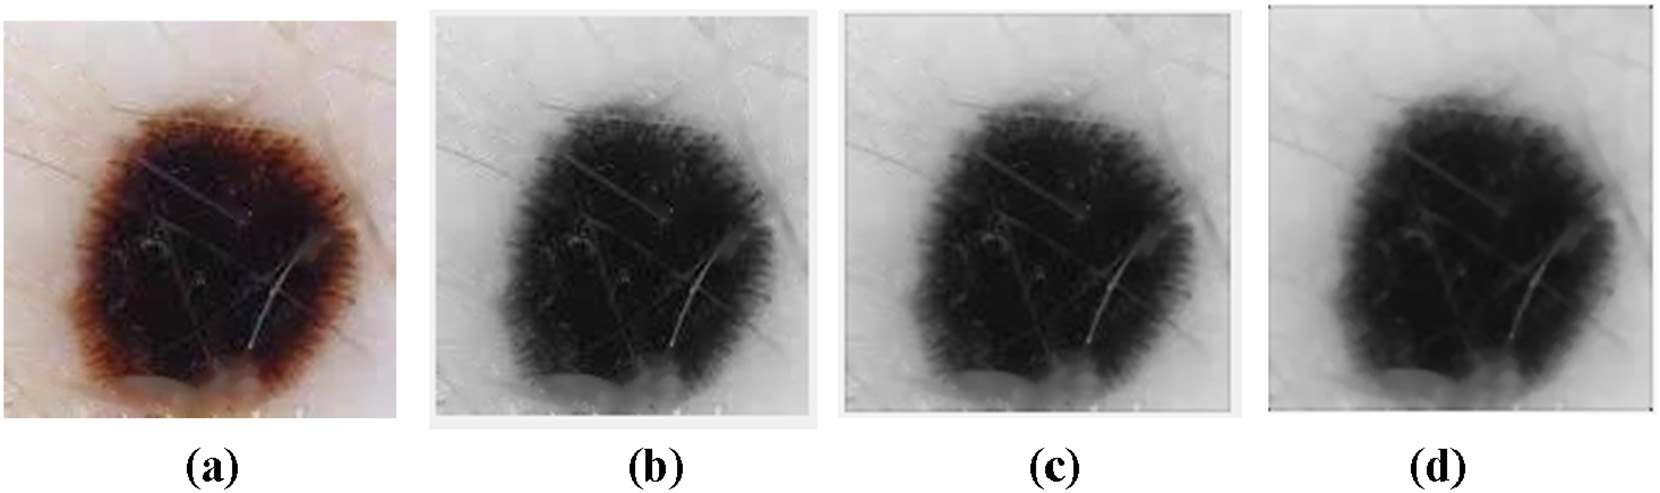
\includegraphics[width=15cm]{./chapter-03-state-of-the-art/preprocessing.png}
\end{center}
\caption{Preprocessing: (a)Dull razor image, (b) Gray scale image, (c) Gaussian filter, (d) Median filter.}
\label{fig:Preprocessing}
\end{figure}




\begin{figure}[htbp]
\begin{center}
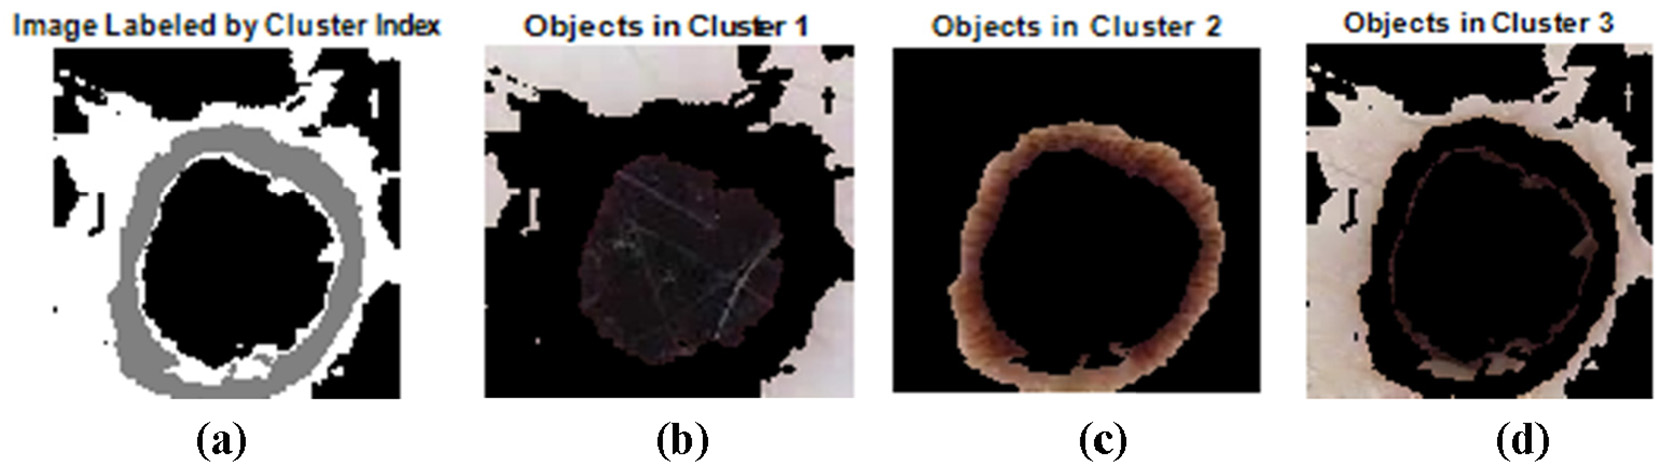
\includegraphics[width=15cm]{./chapter-03-state-of-the-art/segmentation.png}
\end{center}
\caption{Segmentation: (a) Image labelled by cluster index, (b) Objects in cluster 1, (c) Objects in cluster 2, (d) Objects in cluster 3.}
\label{fig:segmentation}
\end{figure}


\begin{figure}[htbp]
\begin{center}
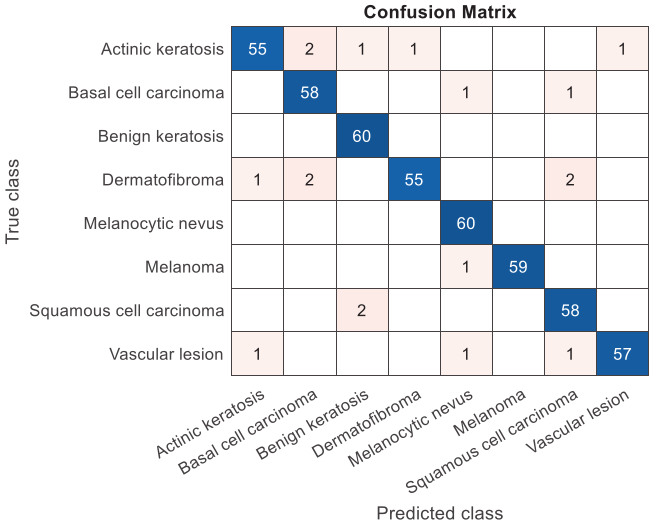
\includegraphics[width=15cm]{./chapter-03-state-of-the-art/confusion-matrix.png}
\end{center}
\caption{Confusion Matrix}
\label{fig:confusion-matrix}
\end{figure}



%=================================================================

\section{Finding reduced Raman spectroscopy fingerprint of skin samples for melanoma diagnosis through machine learning}
    This article ~\cite{Daniella2021} uses a new non-invasive approach to classify malignant and benign tumors, and that is by using Raman spectral data instead of images, Raman Spectroscopy is a way to analyze the chemical structure using light and vibrational energy modes of molecules ~\cite{Edinburgh}.
\begin{description}
\item[Data and method] \hfill \\
    
    \textbf{dataset: }
    For the dataset they brought 33 benign and 51 malignant samples and cut them into regular cuts of $2mm^3$, a laser was used to excite the samples to collect the Raman signals using special tools after this they acquired 436 Raman spectra (spectrum graphs y=f(x) where x is frequency or wave number $cm^-1$ and y is the intensity of scattered light). And they focused on the biological fingerprint spectral region from 800 to 1800 $cm^-1$.

    \textbf{Fluorescence background data pre-processing: }
    Fluorescence is a radiation that is emitted by molecules after interacting with electromagnetic radiation and this could overshadow and disturb the study of Raman spectra, to deal with this noise they used a low frequency laser to lower the probability of fluorescence emissions and by this they could jump the preprocessing step.
\item[Feature extraction] \hfill \\
    They divided the obtained spectrums into subsequences (local spectrums) and extracted some statistical measures from it such as arithmetic mean, standard deviation, derivative ...etc.

\item[Results and discussion] \hfill \\
    These statistical features were then given to a machine learning classification algorithm, a complex decision tree implemented using lightGBM (open source software), other algorithms were also used such as K-nearest neighbors and XGBOOST (Extreme Gradient Boosting an open source software) but the best performance was obtained using lightGBM.
    Further research led them to only use the derivative as a feature and a spectral region from 896 to 1039 $cm^-1$ because these two were proved to have the most discriminative information between malignant and benign tumors and by this they obtained a high performant model ($AUC \geq 0.97$) shown in figure \ref{fig:roc}.
\end{description}

\begin{figure}[htbp]
\begin{center}
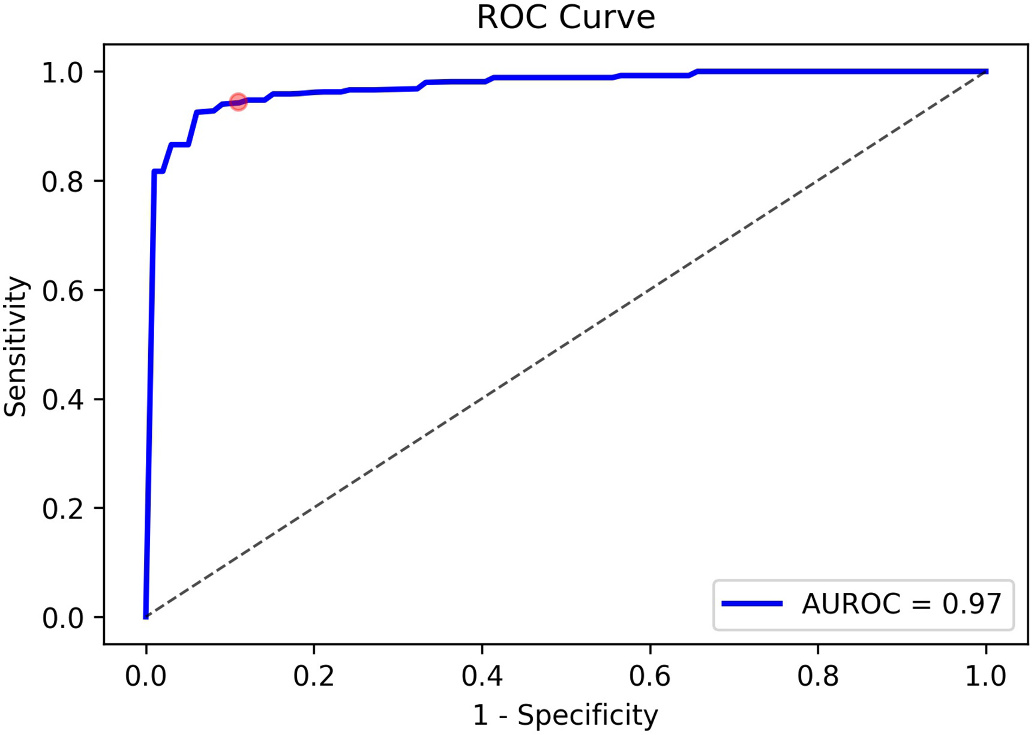
\includegraphics[width=10cm]{./chapter-03-state-of-the-art/ROC.png}
\end{center}
\caption{ROC}
\label{fig:roc}
\end{figure}






%================================================================

\section{Skin cancer detection: Applying a deep learning based model driven architecture in the cloud for classifying dermal cell images}
\begin{description}
\item[Summary] \hfill \\
In this paper ~\cite{Kadampur2020} the researchers are presenting a model driven approach to develop deep learning algorithms for detecting skin cancer by using a tool called DLS (deep learning studio) which is a software that allows you to build deep learning algorithms without being a specialist in programming languages, it presents a simple drag and drop interface for building models it also comes with desktop / cloud versions and community / enterprise editions with multi-GPU training and the possibility to obtain the code of the model, download the model and host it as a REST API (Representational state transfer Application programming interface), the interface dashboard is shown in figure ~\ref{fig:dls}.
\item[Advantage] \hfill \\
The advantage of this non-programmatic approach is for researchers and practitioners to be able to create and test their own models without the need for prior programming knowledge.
\item[Application and Results] \hfill \\
And then they proceed using this tool DLS to show its efficacy and ease of use, they have built and tested 5 models using famous CNN architectures squeeznet, densenet, and inception v3.
With model1 acquiring an AUC of 99.77\% .
\end{description}


\begin{figure}[htbp]
\begin{center}
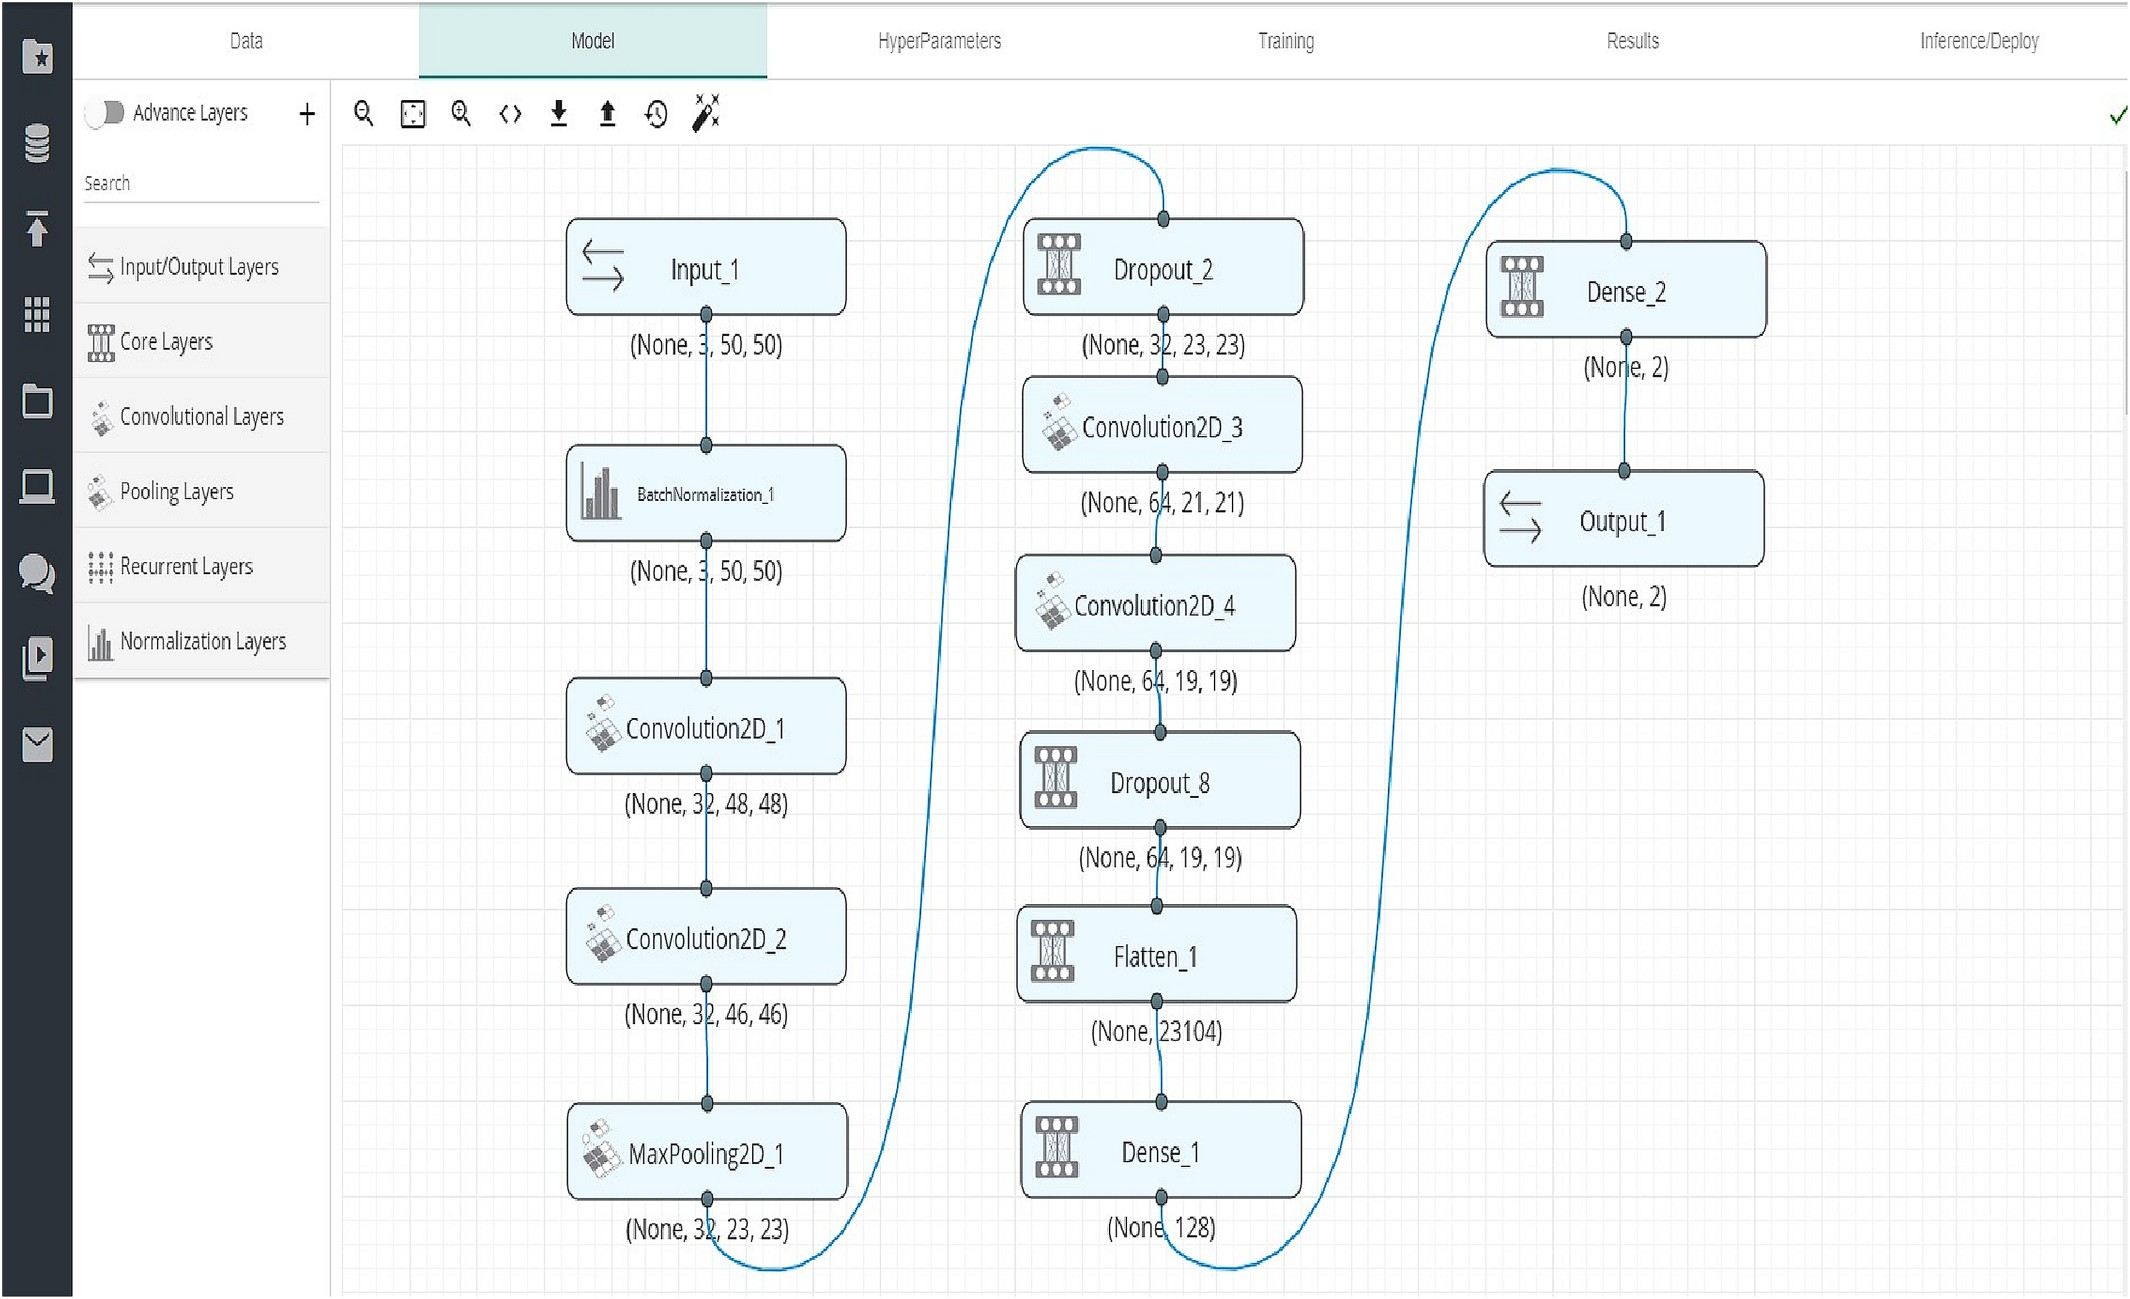
\includegraphics[width=12cm]{./chapter-03-state-of-the-art/dls.png}
\end{center}
\caption{DLS Interface}
\label{fig:dls}
\end{figure}



%========================================================================================


\section{The impact of patient clinical information on automated skin cancer detection}
In this work ~\cite{Pacheco2020} the researchers propose a new idea, which is the use  of clinical information in addition to the image dataset and the study of this addition's effect on the deep learning model's performance.

\begin{description}
\item[Dataset] \hfill \\
To build their hybrid dataset, they proposed a mobile application given to doctors and students to help collect the necessary data from Dermatological Assistance Program (PAD) dataset at the Federal University of Espírito Santo (UFES), which consists of images of the lesion, their clinical diagnosis and 8 clinical information based on common questions that dermatologists ask:
\begin{itemize}
    \item age
    \item part of the body where the lesion is located,
    \item if the lesion itches,
    \item bleeds or has bled,
    \item hurts, 
    \item has recently increased, 
    \item has changed its pattern, 
    \item and if it has an elevation
\end{itemize}

A total of 1612 images of 6 lesions.

Because the image dataset is imbalanced they used multiple strategies to overcome that such as, transfer learning (refining a pretrained model on their dataset), data augmentation, horizontal and vertical rotations, adjusting brightness...etc. and for the clinical data they used one-hot encoding (converting categorical data to augment the performance) which transformed the 8 features collected to an array of 28 values.

\item[Training] \hfill \\
    They used 4 CNN architectures VGGNet-13/19-bn, ResNet-50/101, MobileNet, GoogleNet
    now a problem arose when trying to combine (by concatenation) clinical data with image features extracted by the CNN feature extractor because image features are far more great in size than clinical data, this imbalance is not good for the training and classification because the effect of image features will be greater than the clinical data, that is why they implemented an NN feature reducer on the extracted image features before combining it with the clinical data as shown in figure ~\ref{fig:model}  and the classifier is another neural network that assigns the probabilities for each skin lesion.

\item[Testing the effect of adding clinical data] \hfill \\
    They executed 2 scenarios for that, 1 using models trained only with images, 2 using models trained with images + clinical data then they calculated multiple  performance metrics accuracy, balanced accuracy, weighted precision, weighted recall , weighted F1 score  and area under the curve, and they found almost all models were improved by 7\% in almost all metrics and the best model ResNet-50 presented an $AUC \geq 95.8\%$.

\item[Conclusion] \hfill \\
    Clinical information does make a difference when training ML models to classify skin cancer.
\end{description}



\begin{figure}[htbp]
\begin{center}
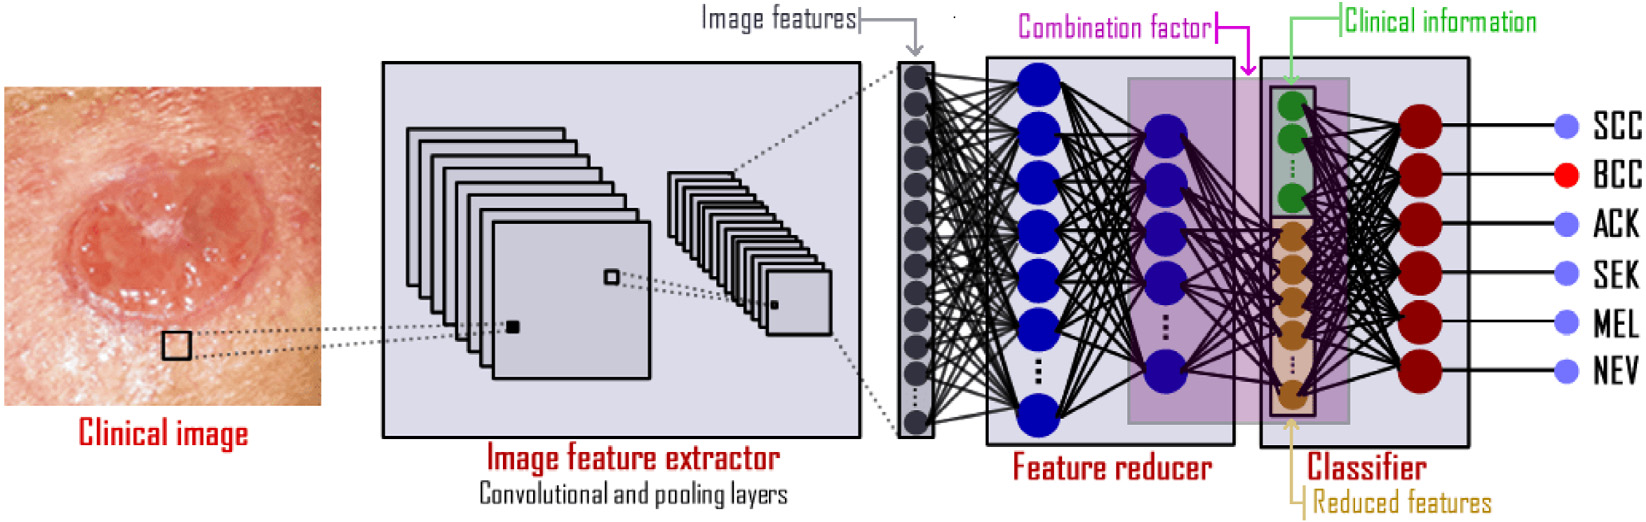
\includegraphics[width=15cm]{./chapter-03-state-of-the-art/clinical-image.png}
\end{center}
\caption{Model}
\label{fig:model}
\end{figure}







%=============================================================================

\section{An artificial neural network based detection and classification of melanoma skin cancer using hybrid texture features}

    In this work ~\cite{Tumpa2021} they try to combine multiple texture features from famous methods such as  ABCD, GLCM and LBP (local binary pattern) and pass all of these features to an ANN (artificial neural network)for learning.

    \begin{description}
    \item [Dataset] \hfill \\
    They preferred to use images captured using a dermatoscope because of their quality over images captured using a phone or normal camera, and they have obtained these images by combining 2 datasets: ISIC archive dataset (jpg format) and PH2 dataset (a dermoscopic image dataset in BMP format) they formed a unified dataset containing 1940 benign and 1448 malignant lesion images.

    \item [Preprocessing] \hfill \\
    Because the images are obtained from various sources, they needed to process them to standardized them in size, shape, format ...etc.
    And also to remove noise and enhance image quality using enhancement algorithms such as histogram equalization process that increases image contrast, and to remove body hair from the images using Maximum Gradient Intensity (MGI) algorithm .

    \item [Image segmentation] \hfill \\
    For better analysis and to remove unwanted parts they segmented the images to keep only the lesion area and for that they used a segmentation method called Otsu's Thresholding .

    \item [Feature extraction] \hfill \\
    They used ABCD (Asymmetry, Border, Color, Diameter), GLCM (energy, contrast, correlation, homogeneity) and LBP (local binary pattern used for textural analysis) as features to train their neural network.

    \item [Classification] \hfill \\
        A feed-forward neural network with backpropagation mechanism is used with the input layer receiving the extracted features and a hidden layer of 100 neurons and an output layer for the final result (1 is malignant and 0 is benign) with biased and weights initialized randomly, Levenberg-Marquardt training and optimization functions are used and while the performance function being Mean Square Error and 2 activation functions "tansig" for the hidden layer and "purelin" for the final output.
        The structure of the ANN is shown in figure ~\ref{fig:ann}.
    
    \item [Evaluation] \hfill \\
        For the evaluation of their classifier they calculated accuracy, specificity, sensitivity and precision shown in figure ~\ref{fig:evaluation}  where all the measures are $>$ 97\%, and furthermore they also studied the effect of each feature on the discrimination process between benign and malignant lesion, and they found that the minimum sensitivity per single feature is 69\%, minimum specificity per single feature is 73\% and minimum accuracy per single feature is 71\% which goes to show that all the used features are playing an important role in the classification process, and lastly they did a comparative evaluation between their work and previous works on the basis of extracted features which showed that more features implies higher performance rates, an example of that is the accuracy of previous works using a combination of some but not all features in (ABCD, GLCM, LBP) always presented an accuracy $<$ 97\%.

    \item [In Conclusion: ] \hfill \\
    The use of hybrid features provided a higher performant model in the detection and classification of benign and malignant melanoma skin cancer.
    \end{description}


\begin{figure}[htbp]
\begin{center}
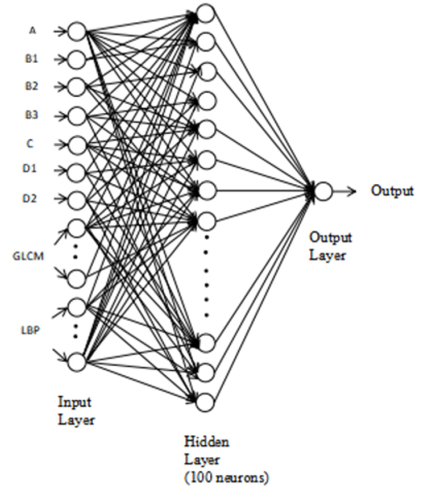
\includegraphics[width=10cm]{./chapter-03-state-of-the-art/ann.png}
\end{center}
\caption{ANN Structure}
\label{fig:ann}
\end{figure}

\begin{figure}[htbp]
\begin{center}
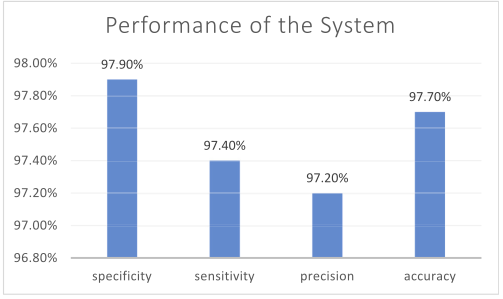
\includegraphics[width=10cm]{./chapter-03-state-of-the-art/evaluation.png}
\end{center}
\caption{Evaluation Measures}
\label{fig:evaluation}
\end{figure}







%=========================================================================


\section{Interpretable deep learning systems for multi-class segmentation and classification of non-melanoma skin cancer}


This article ~\cite{Thomas2021} talks about achieving interpretability in deep learning based systems, and the reason for this is that traditional machine learning models do outperform professionals in some scenarios, but we can't explain their output because they are like black boxes we don't know what is actually going on inside or why the model chose this output instead of another output, so it can not be trusted in high stake situations, for that interpretability of models became a thing in recent research articles, and there are mainly 2 ways in which we can attain interpretability, \textbf{I.)} we can use Model-Agnostic Methods for Interpreting any Machine Learning Model:
\begin{itemize}
    \item like permutation feature importance, 
    \item Partial Dependence Plots (PDPs), 
    \item Individual Conditional Expectation (ICE) plots, 
    \item global surrogate models, 
    \item Local Interpretable Model-agnostic Explanations (LIME) 
    \item Shapley Additive Explanations (SHAP) 
\end{itemize}
To try and explain our model ~\cite{Hennie2020} which are statistical and visual ways used to understand a model, \textbf{II.)} There is another way which is the one used in this article and that is ``naturally interpretable models", which can be defined as models that try to solve the problem the way a human would, which means in the case of skin cancer, analyzing the whole tissue (the same way a doctor would ) and not just cancerous regions of interest, and we can achieve this with semantic segmentation methods.

\begin{description}
\item[Dataset] \hfill \\
    MyLab Pathology provided them with their pre-existing images on non-melanoma cancers, which were taken by a microscope (one image of a cancer is the result of multiple microscopic images concatenated together) for punch, shave and excision biopsies (shave: the surface of the skin is removed with a sharp knife, punch: a round small part of the skin is removed) which meant high resolution images (1px=0.67µm) and each image was annotated by a pathologist to indicate important tissue sections that will be usefull in the classification process, any imbalance of classes was solved using augmentation (rotation and flipping...etc).

\item[Models] \hfill \\
    \begin{description}
    \item[Whole image segmentation] \hfill \\
        input: microscopic image  see figure ~\ref{fig:seg-input}. \hfill \\
        ouput: h x w x 12 (12 probability distribution maps), see figure ~\ref{fig:seg-output}.  \hfill \\
        the different tissue sections were colored 
        \begin{enumerate}
            \item Glands (GLD) 
            \item Inflammation (INF) 
            \item Hair Follicles (FOL) 
            \item Hypodermis (HYP) 
            \item Reticular Dermis (RET) 
            \item Pap-illary Dermis (PAP) 
            \item Epidermis (EPI) 
            \item Keratin (KER) 
            \item Background (BKG) 
            \item BCC (Basal cell carcinoma)
            \item SCC (Squamous cell carcinoma)
            \item IEC (a very early treatable form of skin cancer)
        \end{enumerate}
        To be fed to the segmentation model to train on semantic segmentation, this model was created using a combination of U-net-like architecture (U-net: a famous CNN architecture for biomedical image segmentation) and a pretrained headless ResNet50 network. Because of the high resolution of the microscopic images they were fed to the model in parts of 256x256 and 512x512 pixels.

    \item[Whole image classification] \hfill \\

        Input: output of segmentation (h x w x [12 images]). \hfill \\
        Output: 4 classes Healthy, BCC, SCC and IEC. \hfill \\
        The output of whole image segmentation (which was a probability distribution for each pixel on the 12 tissue classes) was fed to a CNN to train as a classifier using Adam optimizer (used to accelerate the gradient descent algorithm) and a learning rate of 0.0001, with a ratio of 80:10:10 for training, validation and testing.
    \end{description}


\item[Results and discussion] \hfill \\
    The segmentation model achieved a per-pixel accuracy of 86\% and overall class accuracy of 85\%, they found that downgrading the image's size before training to 10 times less increases the accuracy but only by a little bit ~2\% which isn't much, but this information is still useful because it means that we can use low resolution images and still get a high performant model with less computational power.

    The classification model achieved an accuracy of 93.6\% over the 4 classes compared to other algorithms trained with the same data such as (Random Forest 87.2\%, KNN 80.9\%, Single-layer Perceptron 85.1\%).


\item[Conclusion] \hfill \\
    They showed that in order to build an interpretable model for skin cancer detection and classification you need to train your model the same way a real doctor would try to diagnose the skin cancer, and they did that by feeding and training the algorithm with the same data a dermatologist would use for diagnosis without ignoring anything such as hair, sweat glands ...etc. In the end they obtained a high performant model that is interpretable (which means that when a doctor sees the classification of the algorithm he can understand why it chose that classification) which will increase the possibility to use this approach in real life high stake scenarios, furthermore, because they used a diverse dataset they said their algorithm can be used for more routine work that a dermatologist would do such as assessing aggressiveness, depth, direction of growth and even calculating surgical margins (to know how much tissue to remove to guarantee that all cancerous cells are removed).
\end{description}



\begin{figure}[h]
\centering
    \begin{subfigure}[b]{0.3\textwidth}
        \centering
        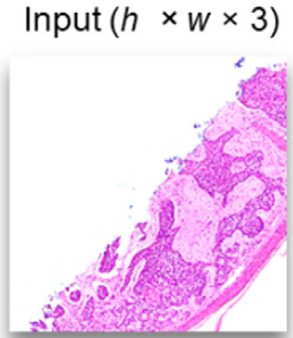
\includegraphics[scale=.5]{./chapter-03-state-of-the-art/seg-input.png}
        \caption{Input}
        \label{fig:seg-input}
    \end{subfigure}
    \begin{subfigure}[b]{0.3\textwidth}
        \centering
        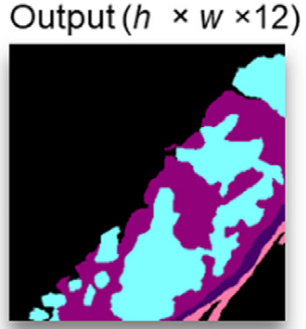
\includegraphics[scale=.5]{./chapter-03-state-of-the-art/seg-output.png}
        \caption{Output}
        \label{fig:seg-output}
    \end{subfigure}
\caption{Whole segmentation model input and output}
\label{fig:seg-input-output}
\end{figure}





% \begin{figure}[htbp]
% \begin{center}
% 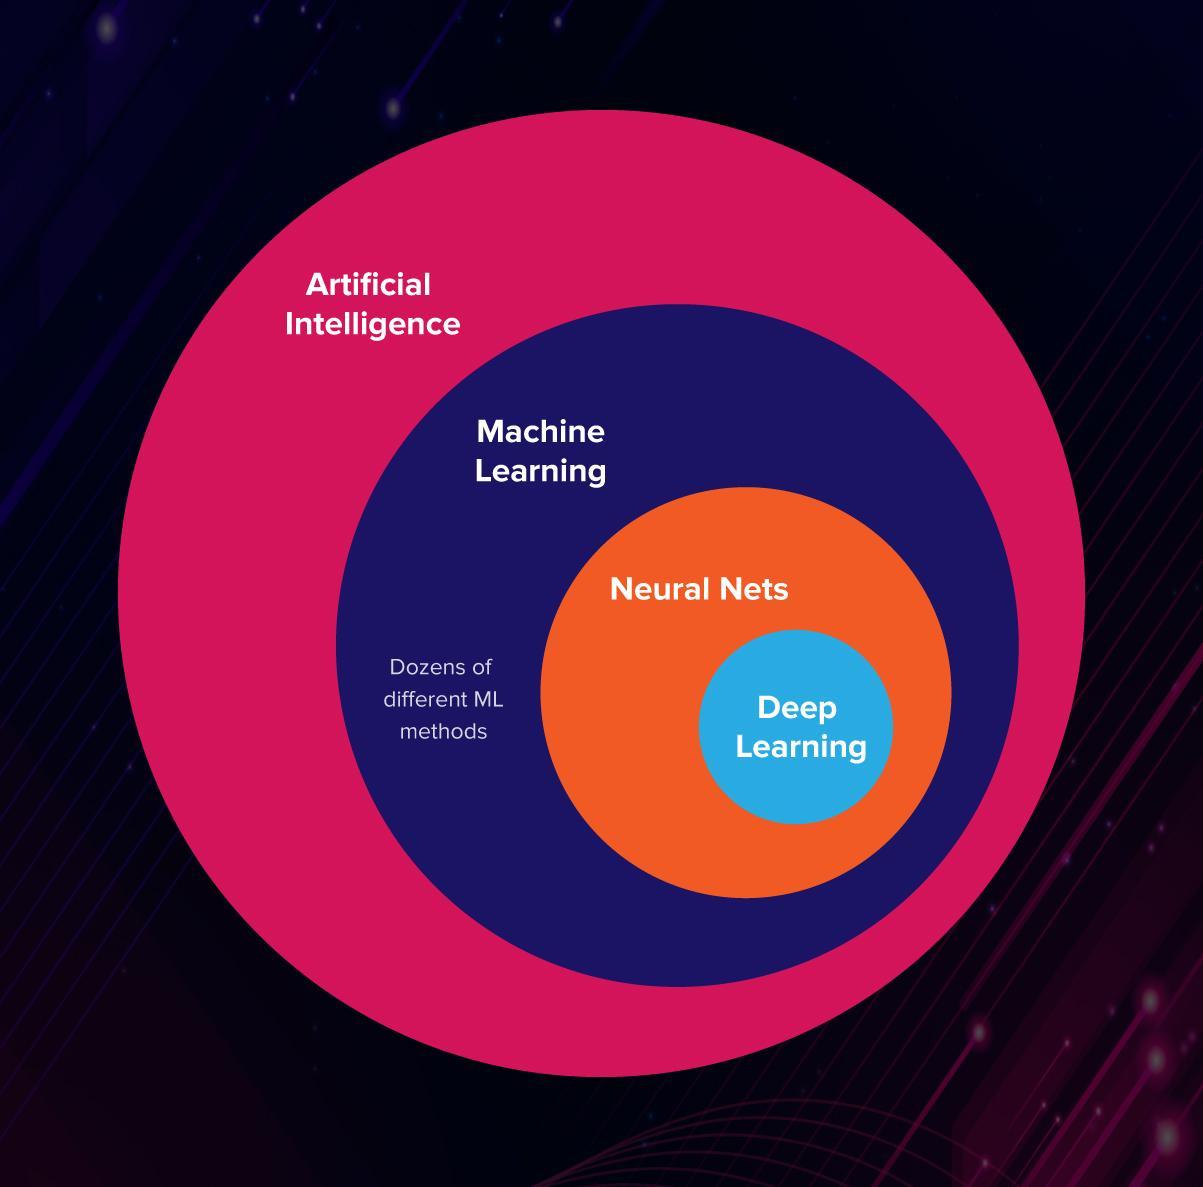
\includegraphics[width=2cm]{./chapter-03-state-of-the-art/versus.jpg}
% \end{center}
% \caption{}
% \label{fig:}
% \end{figure}

\section{Comprehensive Comparative Information}
In this section we are going to present a comprehensive comparative information for the various methods tested on benchmark datasets and their evaluation metrics that were extracted from previous literature work, we present these tables as a recap since all the methods pass through the same steps (dataset, preprocessing, feature extraction and prediction), we present a table ~\ref{tab:outable} that recaps the methods  mentioned above and 2 more tables with other methods ~\ref{tab:first} ~\ref{tab:second}, and it is also worth mentioning that the best methods used in the last 6 years (2016, 2021) using KPI-accuracy are SVM in machine learning and CNN in deep learning and the utilization shares are 54\% for ML methods and 46\% for DL methods ~\cite{Painuli2022}.
% \bigskip


\begin{table}[htbp]
    \begin{center}
        \begin{tabular}{p{3cm}|p{3cm}|p{6cm}}
        \hline 
        Method & Dataset & Results  \\ 
        \hline 
        classification using MSVM & 800 dermoscopic images ISIC of 8 lesion &  accuracy 96.25\% \\ 
        \hline 
        classification using lightGBM (complex decision tree) & 436 Raman spectra (x:frequency, y:intensity of scattered light) for benign and malignant & AUC $>$ 97\%  \\ 
        \hline 
        CNN famous architectures (implemented using deep learning studio) & Kaggle image dataset &   AUC 99\% \\ 
        \hline 
        classification using multiple CNN architectures & images (1612 images of 6 lesions)+ clinical info &  AUC 95.8\% and clinical added a 7\% to almost all performance metrics \\ 
        \hline 
        binary classification ANN & hybrid features ABCD, GLCM, LBP from dermoscopic  ISIC+PH2 datasets (1940 benign + 1448 malignant) & performance measures all $>$ 97\%, effect of each feature $>$ 69\%  \\ 
        \hline 
        segmentation to 12 tissue classes CNN (U-net, Resnet) and CNN classification (healthy and 3 lesions) & MyLab Pathology provided access to their pre-existing collection of skin cancer slides & 93.6\% accuracy compared to (Random Forest 87.2\%, KNN 80.9\%, Single-layer Perceptron 85.1\%) \\ 
        \hline 
        \end{tabular} 
    \end{center}
\caption{A comparative table of the methods mentioned above in this article}
\label{tab:outable}
\end{table}

\begin{table}[htbp]
    \begin{center}
        \begin{tabular}{p{3cm}|p{3cm}|p{6cm}}
        \hline 
        Method & Dataset & Results  \\ 
        \hline 
         DCNN & PH2/ISBI 2016/ISBI 2017 & 98.4\% on PH2 dataset, 95.1\% on ISBI dataset and 94.8\% on ISBI 2017 dataset \\ 
        \hline 
         GLCM features to an SVM & ISIC & 95\% (Accuracy) 90\% (sensitivity) 85\% (specificity) \\ 
        \hline 
            hybrid adaboost SVM  & Skin Cancer and Benign Tumor Image Atlas-Contents & 91.7\% (Accuracy) 94.1\%(sensitivity) 88.7\%(specificity) 0.83\%(Kappa) \\ 
        \hline 
            ABCD features to an SVM & PH2 & 90.63\% (Accuracy) 95\% (sensitivity) 83.33\%(specificity) \\ 
        \hline 
         FCRN architecture & ISIC & 0.912\%(AUC) 0.857\% (Accuracy) 0.490\%(sensitivity) 0.961\%(specificity) 0.729\%(average precision) \\ 
        \hline 
         ANN & ISIC & 74.76\% (Accuracy) 57.56\% (validation loss) \\ 
        \hline 
         CNN & Large collection of Multi-Source Dermatoscopic Images & 75.2 (Accuracy) 0.71 (validation loss) \\ 
        \hline 
        \end{tabular} 
    \end{center}
\caption{A comparative table of the latest methods used in skin lesion detection. DCNN(Deep convolutional neural network), FCRN (Fully Convolutional Residual Networks) ~\cite{Saba2020}}
\label{tab:first}
\end{table}






\small
    \begin{longtable}{p{4cm}|p{4cm}|p{6cm}}
        % \label{tab:}
        \hline
        \multicolumn{3}{| c |}{Beginning}\\
        \hline
        Method and Dataset & Results & Limitations  \\   
        \hline
        \endfirsthead

        \hline
        \multicolumn{3}{| c |}{Continuation}\\
        \hline
        Method and Dataset & Results & Limitations  \\   
        \hline
        \endhead

        \hline
        \endfoot

        \endlastfoot
       
        \hline
        ResNet/ Hallym dataset 19,398 instances are used & For Basal Cell Carcinoma (BCC)/ 96\% for asian dataset/ 90\% for the instances of Caucasian for Melanoma –/ 96\% for the instance of Asian/ 88\% for Caucasian dataset & Model performance depends on patient ethnicity \\
        \hline
        Whale algorithm applied to optimize the CNN model/ Around 22,000 images of Dermquest and DermIS dataset were used & Achieved :/ Specificity 98\%/ Accuracy- 94\%/ Sensitivity-97\%/ PPV-90\% & Results are unsatisfactory for non–Melanoma cases \\
        \hline
        ResNet/ Clinical images/ Clinical data are included & Achieved :/ 67.1\% for clinical images/ 78.8\% for clinical data and images & Missing values are not handled in clinical data/ Biopsy images are not included \\
        \hline
        ResNet/ 1279 dermoscopic instances are used & Achieved 89.2\% for ResNet without dermatologist/ 94.3\% for ResNet- with dermatologist & Clinical information to be included/ No standard evaluation criteria exist to measure classification efficacy \\
        \hline
        ResNet/ HAM10000 dataset, ISIC archive- 11,444 dermatoscopic instances are used & Mean accuracy of/ Physician 42.94/ CNN model – 81.59/ Fusion model – 82.59 & Model outperformed for the trained dataset, but performance degraded for other datasets. \\
        \hline
        ResNet/ Dermnet dataset provides an instance of 23 categories of skin diseases & Achieved 97.1\% & Able to identify few skin diseases like/ Acne , Rosacea, Hemangioma,/ Psoriasis, Seborrheic Dermatitis\\
        \hline
        Dragonfly optimized DNN model is assessed using existing techniques such as Support Vector Machine, ANN, and to display the efficiency of the system diverse evaluation criteria’s are accuracy, sensitivity, and specificity are considered & Achieved/ Sensitivity – 84\%/ Specificity- 99.5\%/ Accuracy – 98.5\% & Result generated for Melanoma is inadequate\\
        \hline
        CNN model used to categorized the skin cancer into Melanoma, nevi, basal cell carcinoma/ 11,444 dermoscopic images HAM10000 dataset, ISIC archive was used & 89.2\% of specificity and 56.5\% of sensitivity attained by the dermatologists/ Whereas the CNN model achieved 98.8\% of sensitivity, and specificity & Model biased and failed to classify skin lesion properly/ For melanoma images CNN model diagnosed it as nevi whereas dermatologists diagnosed it as melanoma/ model achieved the lowest specificity 94.2\% for melanoma class\\
        \hline
        GoogleNet CNN model/ 4800 clinical images & Achieved/ Sensitivity 96.3\% Specificity 59.5\% & Model behavior depends on skin color tone, and Model biased, sensitivity and specificity dropped for Caucasian patients/ No standard evaluation criteria exist to measure classification efficacy\\
        \hline
        DenseNet, ResNet model results compared with Dermatologist/ 10,135 dermoscopy images of HAM10000: 10015, PH2: 120 data sets are used & For Melanoma and BCC – achieved94.40\% for ResNet, 99.30\% for DenseNet whereas Dermatologist achieved – 82.26\% and 88.82\% accuracy & Model biased for the diverse dataset/ Model behavior depends on skin tone colour\\
        \hline
        \caption{Another comparative table of the latest methods used in skin lesion detection and their limitations ~\cite{Naresh2020}}
        \label{tab:second}
    \end{longtable} 
 
